\section{ИССЛЕДОВАНИЕ РАБОТЫ JK-ТРИГГЕРА}

\begin{figure}[H]
	\centering
	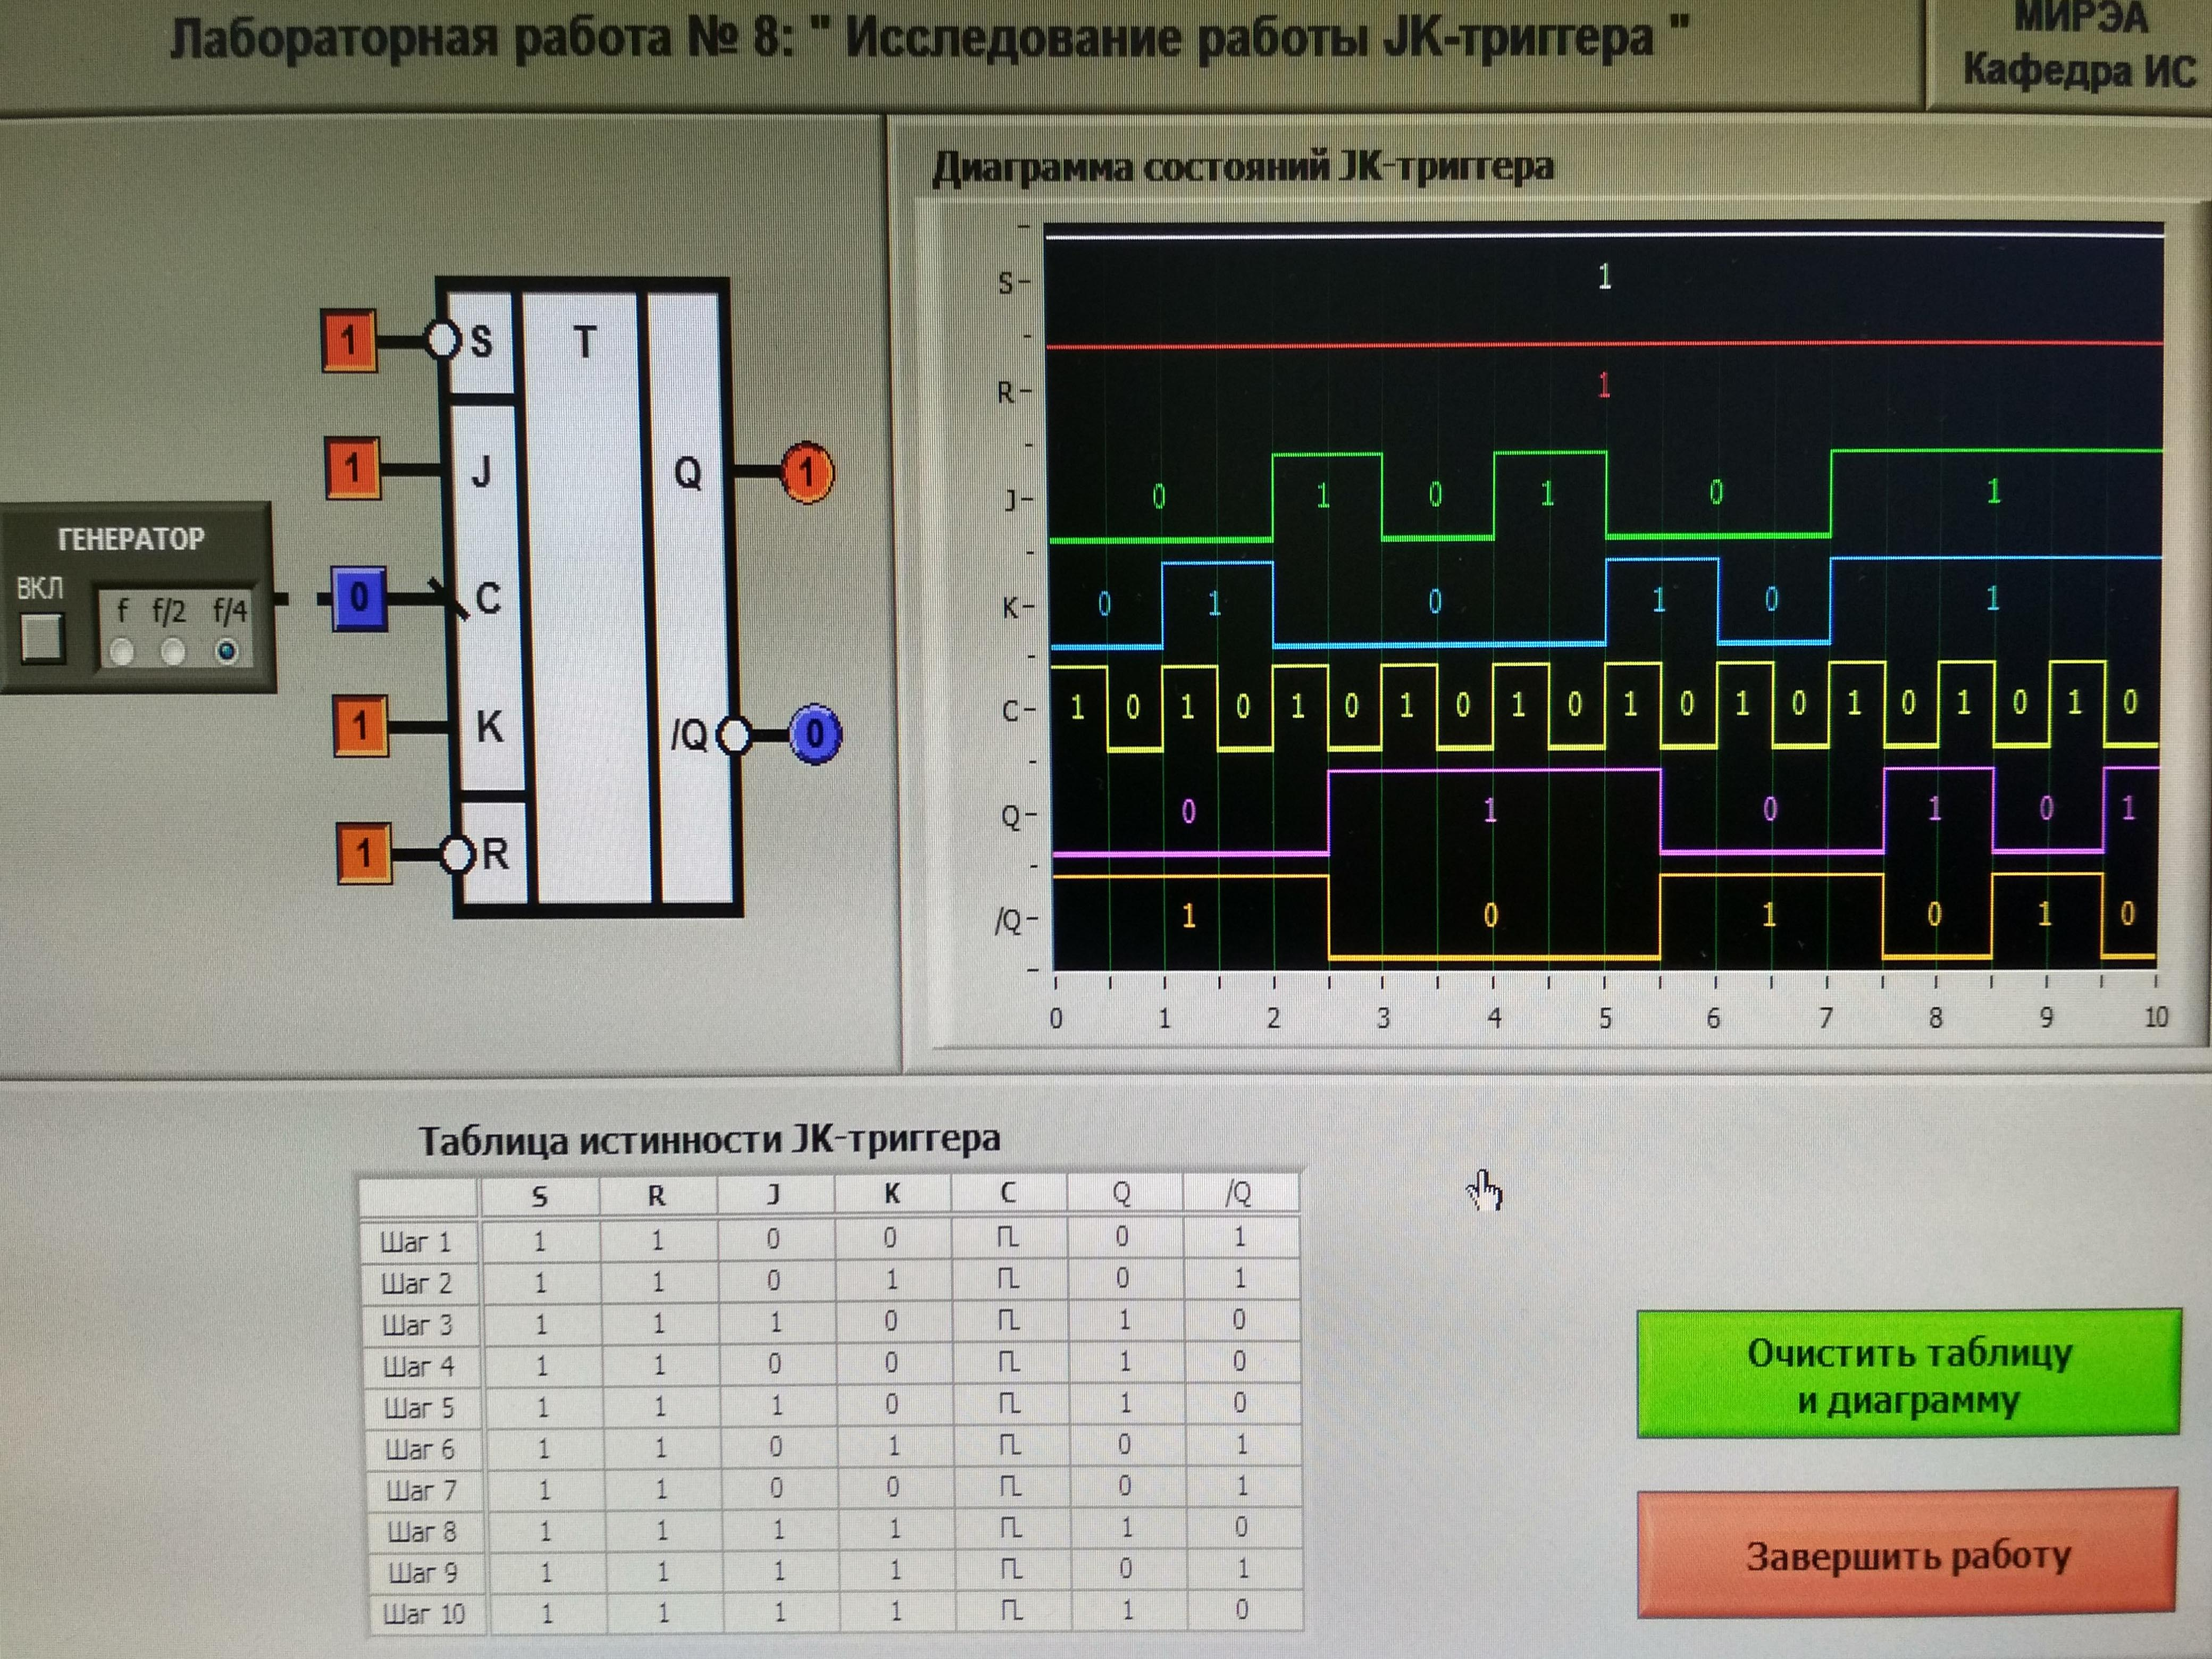
\includegraphics[width=0.95\linewidth]{imgs/8/1}
	\caption{Результат работы JK-триггера}
	\label{fig:8_1}
\end{figure}

\begin{table}[H]
	\centering
	\caption{Переключение состояния JK-триггера}
	\label{tab:lab_08_states}
	\begin{tabular}{|c|c|c|c|}
		\hline
		Выход $Q_n$ & Вход J   & Вход K   & Выход $Q_{n+1}$ \\ \hline
		0           & $\times$ & 0        &                 \\ \hline
		0           & 0        & 1        & 0               \\ \hline
		1           & 1        & 0        & 1               \\ \hline
		1           & 0        & $\times$ &                 \\ \hline
	\end{tabular}
\end{table}

\begin{table}[H]
	\centering
	\caption{Список состояний JK-триггера}
	\label{tab:lab_08_mode}
	\begin{tabular}{|c|c|c|}
		\hline
		Режим работы        & Вход J & Вход K \\ \hline
		Хранение информации & 0      & 0      \\ \hline
		Установка 1         & 1      & 0      \\ \hline
		Установка 0         & 0      & 1      \\ \hline
		Переключение        & 1      & 1      \\ \hline
	\end{tabular}
\end{table}

\begin{figure}[H]
	\centering
	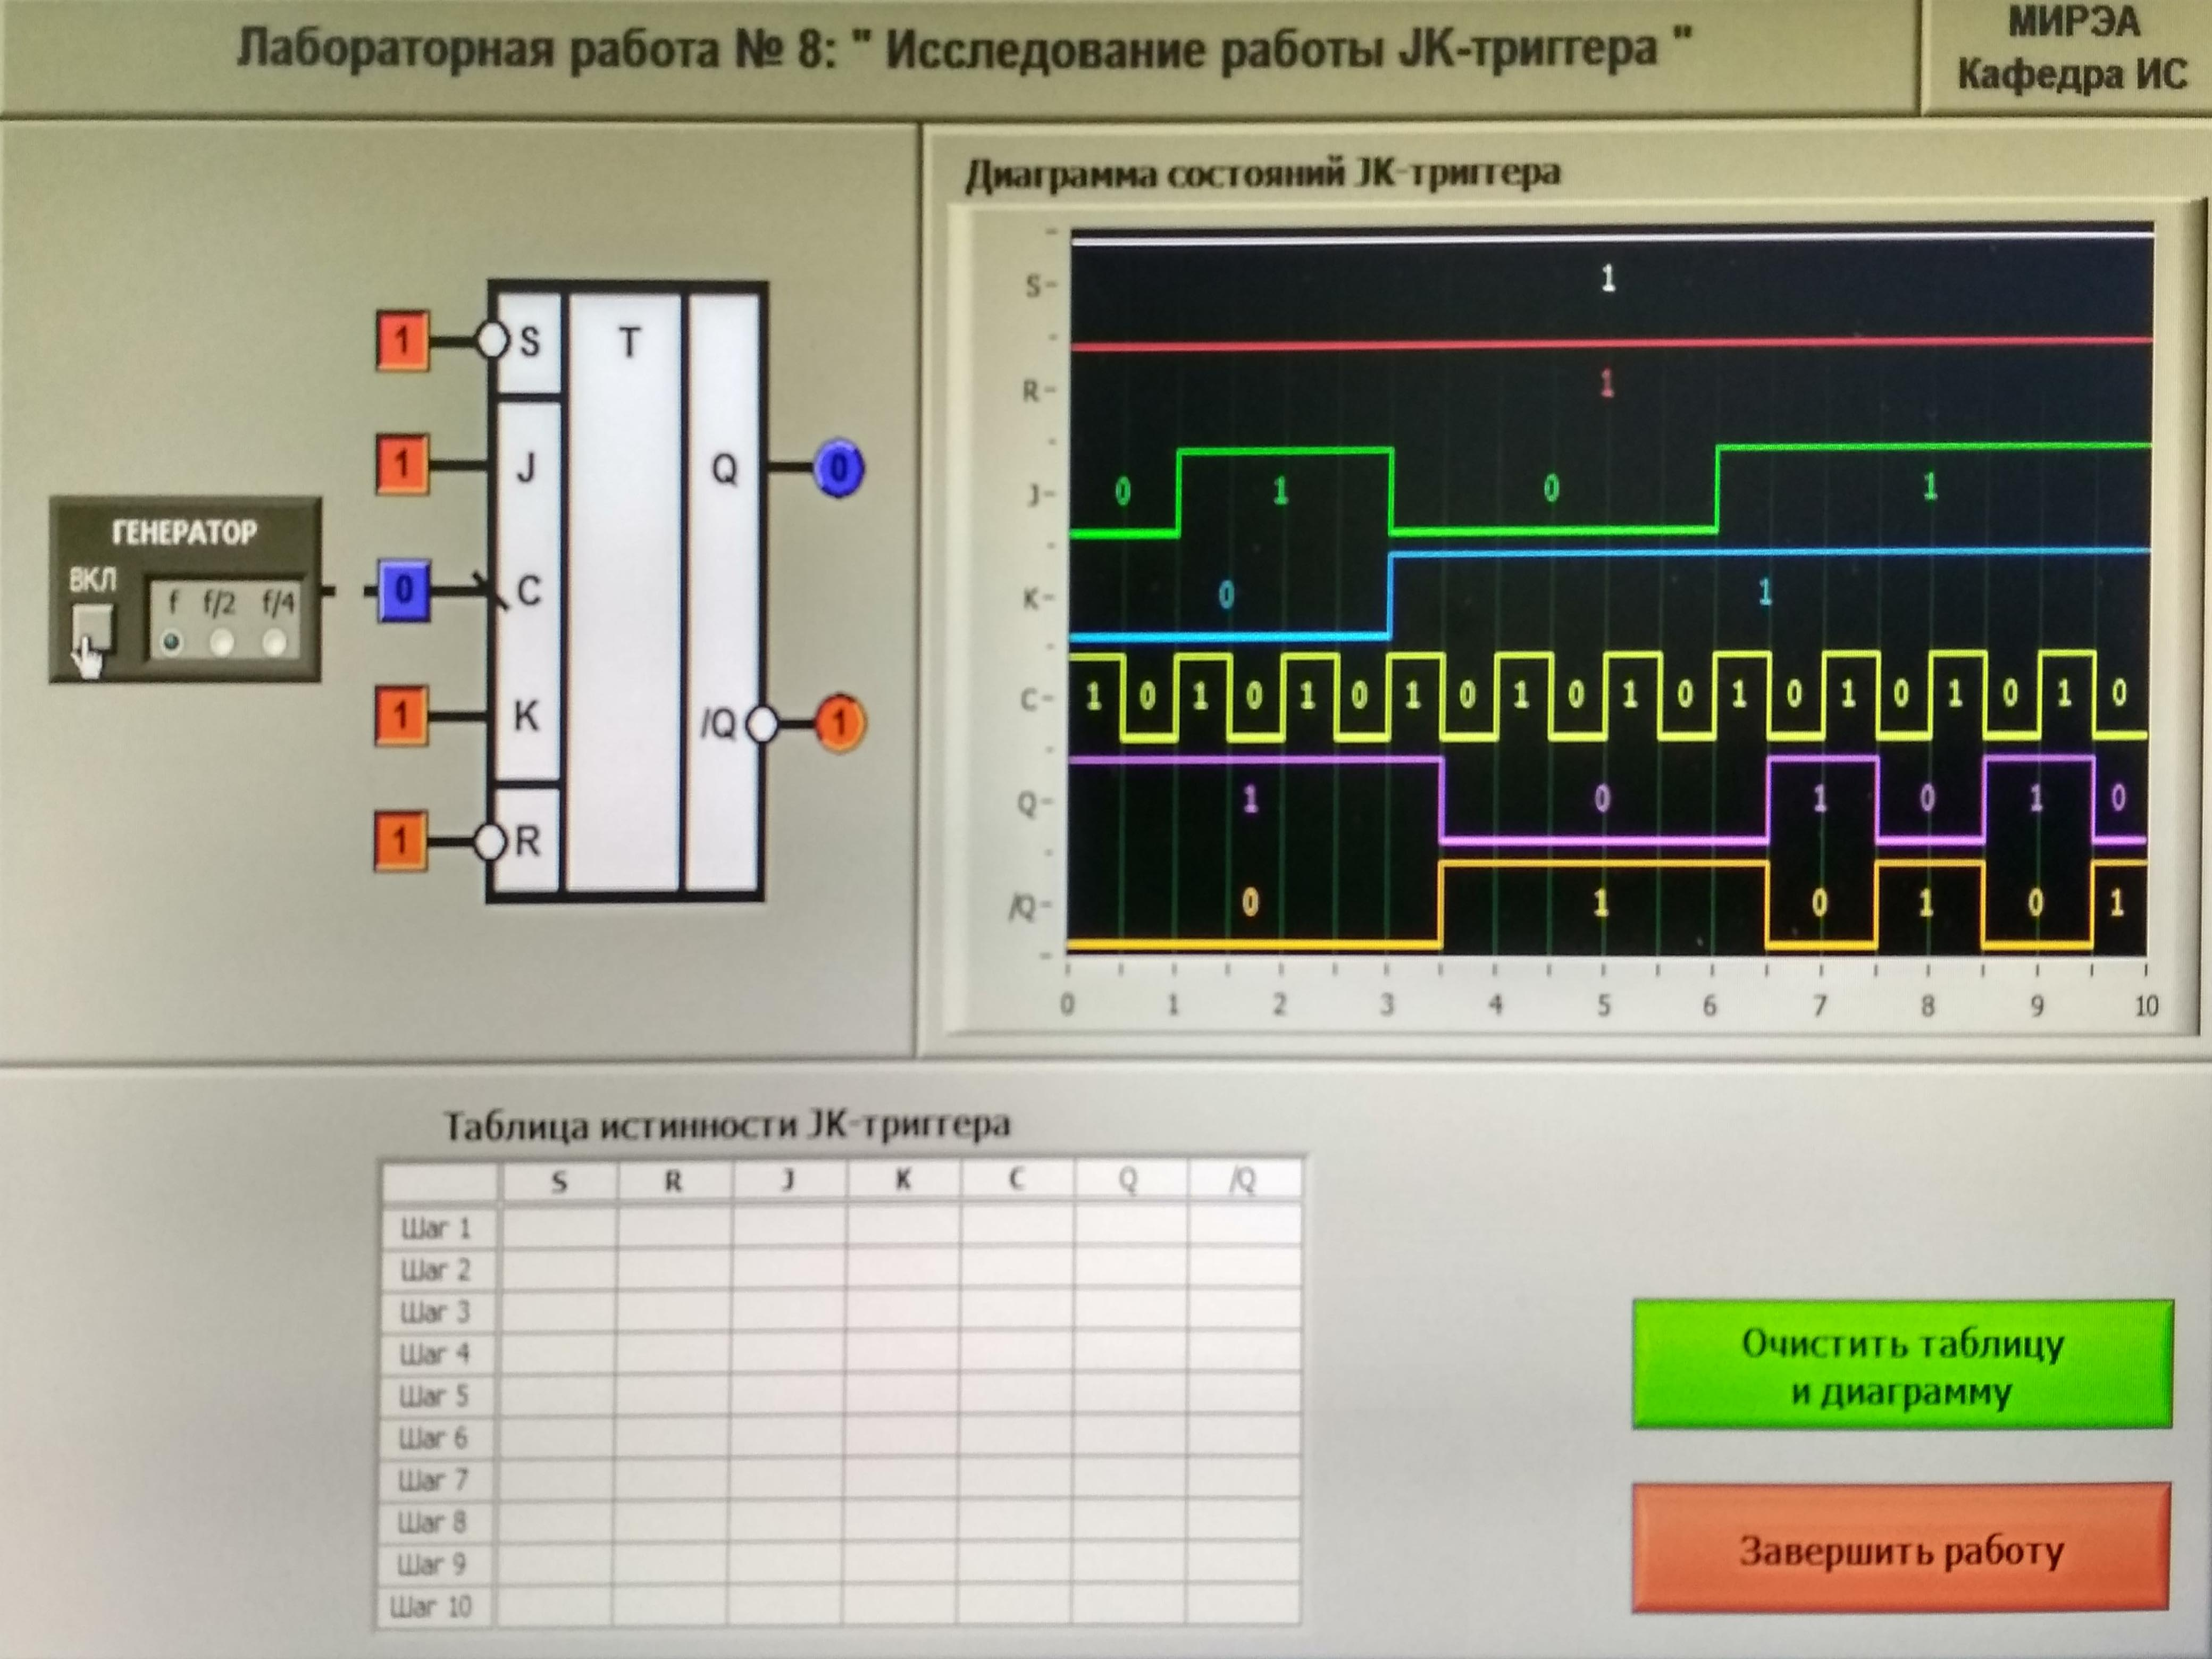
\includegraphics[width=0.95\linewidth]{imgs/8/2}
	\caption{Результат работы JK-триггера в режиме генератора}
	\label{fig:8_2}
\end{figure}

Элемент SN54HC109-SP - High-Speed CMOS

Характеристики:

\begin{figure}[H]
	\centering
	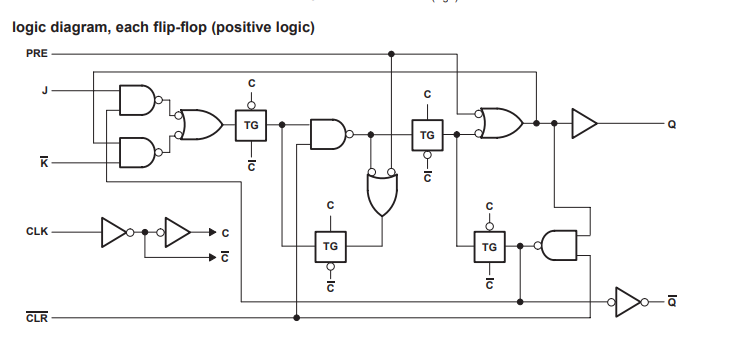
\includegraphics[width=0.95\linewidth]{imgs/8/ti1}
	\caption{Логическая схема}
	\label{fig:8_ti1}
\end{figure}

\begin{figure}[H]
	\centering
	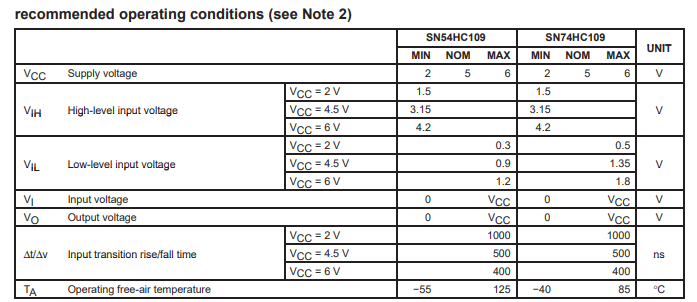
\includegraphics[width=0.95\linewidth]{imgs/8/ti2}
	\caption{Рекомендуемые параметры}
	\label{fig:8_ti2}
\end{figure}

\begin{figure}[H]
	\centering
	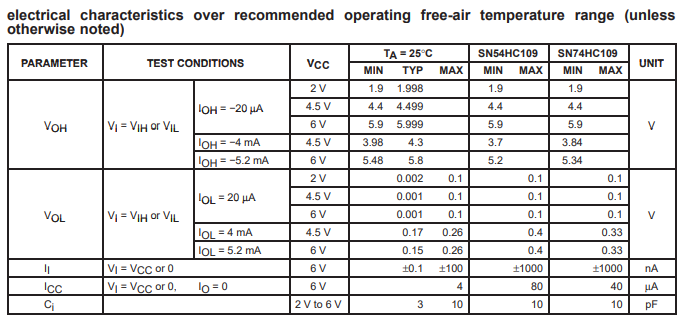
\includegraphics[width=0.95\linewidth]{imgs/8/ti3}
	\caption{Электрические характеристики}
	\label{fig:8_ti3}
\end{figure}

\begin{figure}[H]
	\centering
	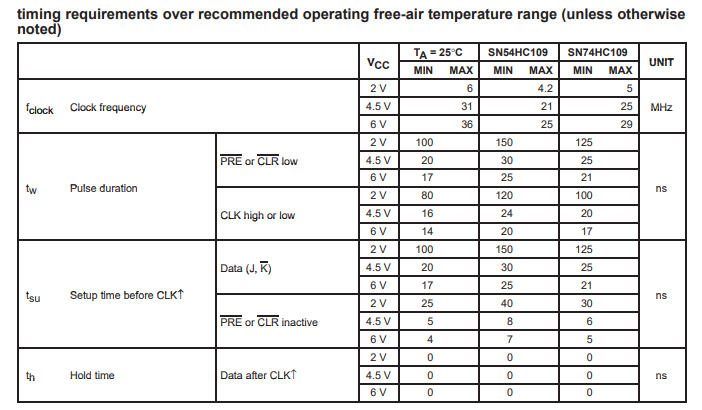
\includegraphics[width=0.95\linewidth]{imgs/8/ti4}
	\caption{Время задержек}
	\label{fig:8_ti4}
\end{figure}

\begin{figure}[H]
	\centering
	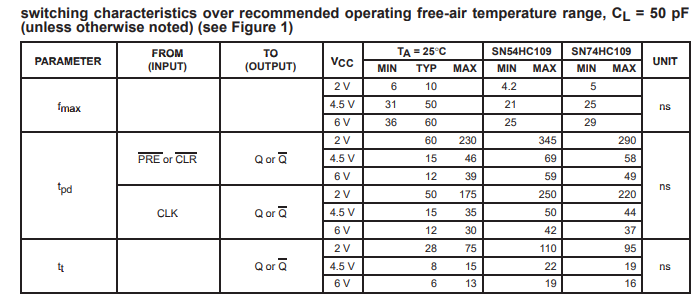
\includegraphics[width=0.95\linewidth]{imgs/8/ti5}
	\caption{Время переключения}
	\label{fig:8_ti5}
\end{figure}